%%%%%%%%%%%%%%%%%%%%%%%%%%%%%%%%%%%%%%%%%
% Beamer Presentation
% LaTeX Template
% Version 1.0 (10/11/12)
%
% This template has been downloaded from:
% http://www.LaTeXTemplates.com
%
% License:
% CC BY-NC-SA 3.0 (http://creativecommons.org/licenses/by-nc-sa/3.0/)
%
%%%%%%%%%%%%%%%%%%%%%%%%%%%%%%%%%%%%%%%%%

%----------------------------------------------------------------------------------------
% PACKAGES AND THEMES
%----------------------------------------------------------------------------------------

\documentclass[10pt,xcolor={dvipsnames}]{beamer}
%\setbeamersize{text margin left=1em,text margin right=1em}
\usepackage{mathtools}
\usepackage{amsmath}
\usepackage{bm}
\usepackage{hyperref}

\usepackage{graphicx} % Allows including images
\graphicspath{{/Users/rebecca/Documents/Rivet_Analyses/MC_VBFDM/PlotCombinationTool/Figures/}{/Users/rebecca/Documents/Presentations/Talks/}}
\usepackage{booktabs} % Allows the use of \toprule, \midrule and \bottomrule in tables

\usepackage{etoolbox}

\usepackage{subcaption}
\captionsetup{compatibility=false}

\usepackage{multirow}

\usepackage{appendixnumberbeamer}

%\newlength\origleftmargini
%\setlength\origleftmargini\leftmargini
%\setbeamertemplate{itemize/enumerate body begin}{\setlength{\leftmargini}{2pt}}%

%\let\oldexampleblock\exampleblock
%\let\oldendexampleblock\endexampleblock
%\def\exampleblock{\begingroup \setbeamertemplate{itemize/enumerate body begin}{\setlength{\leftmargini}{\origleftmargini}} \oldexampleblock}
%\def\endexampleblock{\oldendexampleblock \endgroup}%

%\let\oldalertblock\alertblock
%\let\oldendalertblock\endalertblock
%\def\alertblock{\begingroup \setbeamertemplate{itemize/enumerate body begin}{\setlength{\leftmargini}{\origleftmargini}} \oldalertblock}
%\def\endalertblock{\oldendalertblock \endgroup}

\mode<presentation> {

% The Beamer class comes with a number of default slide themes
% which change the colors and layouts of slides. Below this is a list
% of all the themes, uncomment each in turn to see what they look like.

%\usetheme{default}
%\usetheme{AnnArbor}
%\usetheme{Antibes}
%\usetheme{Bergen}
%\usetheme{Berkeley}
%\usetheme{Berlin}
\usetheme{Boadilla}
%\usetheme{CambridgeUS}
%\usetheme{Copenhagen}
%\usetheme{Darmstadt}
%\usetheme{Dresden}
%\usetheme{Frankfurt}
%\usetheme{Goettingen}
%\usetheme{Hannover}
%\usetheme{Ilmenau}
%\usetheme{JuanLesPins}
%\usetheme{Luebeck}
%\usetheme{Madrid}
%\usetheme{Malmoe}
%\usetheme{Marburg}
%\usetheme{Montpellier}
%\usetheme{PaloAlto}
%\usetheme{Pittsburgh}
%\usetheme{Rochester}
%\usetheme{Seahorse}
%\usetheme{Singapore}
%\usetheme{Szeged}
%\usetheme{Warsaw}

% As well as themes, the Beamer class has a number of color themes
% for any slide theme. Uncomment each of these in turn to see how it
% changes the colors of your current slide theme.

%\usecolortheme{albatross}
%\usecolortheme{beaver}
%\usecolortheme{beetle}
%\usecolortheme{crane}
%\usecolortheme{dolphin}
%\usecolortheme{dove}
%\usecolortheme{fly}
%\usecolortheme{lily}
%\usecolortheme{RoyalBlue}
%\usecolortheme{rose}
%\usecolortheme{seagull}
%\usecolortheme{seahorse}
%\usecolortheme{whale}
%\usecolortheme{wolverine}

%%Changing the theme colours
%\setbeamercolor*{structure}{bg=Plum!20,fg=Plum}
%\setbeamercolor*{palette primary}{use=structure,fg=white,bg=structure.fg}
%\setbeamercolor*{palette secondary}{use=structure,fg=white,bg=structure.fg!75}
%\setbeamercolor*{palette tertiary}{use=structure,fg=white,bg=structure.fg!50!black}
%\setbeamercolor*{palette quaternary}{fg=white,bg=black}
%\setbeamercolor{section in toc}{fg=black,bg=white}
%%\setbeamercolor{alerted text}{use=structure,fg=structure.fg!50!black!80!black}
%\setbeamercolor{titlelike}{parent=palette primary,fg=structure.fg!50!black}
%\setbeamercolor{frametitle}{bg=gray!30!white,fg=Plum}
%\setbeamercolor*{titlelike}{parent=palette primary}

%Changing the theme colours
\setbeamercolor*{structure}{bg=RoyalPurple,fg=RoyalPurple}
\setbeamercolor*{palette primary}{use=structure,fg=white,bg=structure.fg}
\setbeamercolor*{palette secondary}{use=structure,fg=white,bg=structure.fg}
\setbeamercolor*{palette tertiary}{use=structure,fg=white,bg=structure.fg}
\setbeamercolor*{palette quaternary}{fg=white,bg=black}
\setbeamercolor{section in toc}{fg=black,bg=white}
%\setbeamercolor{alerted text}{use=structure,fg=structure.fg!50!black!80!black}
\setbeamercolor{titlelike}{parent=palette primary,fg=structure.fg!50!black}
%\setbeamercolor{frametitle}{use=structure,fg=white,bg=structure.fg}
\setbeamercolor*{titlelike}{parent=palette primary}

%\setbeamercolor{block}{bg=yellow!10,fg=black}
%\setbeamercolor{block title}{bg=yellow!50,fg=black}
%\AtBeginEnvironment{block}{\setbeamercolor{itemize item}{fg=yellow}}

\newenvironment<>{examplefirst}[1]{%
  \setbeamercolor{block title}{bg=yellow!50,fg=black}%
  \begin{block}#2{#1}}{\end{block}}
\AtBeginEnvironment{examplefirst}{\setbeamercolor{itemize item}{fg=yellow}}

%\setbeamertemplate{footline} % To remove the footer line in all slides uncomment this line
%\setbeamertemplate{footline}[page number] % To replace the footer line in all slides with a simple slide count uncomment this line

%\setbeamertemplate{navigation symbols}{} % To remove the navigation symbols from the bottom of all slides uncomment this line


\setbeamertemplate{blocks}[rounded][shadow=false]
\setbeamertemplate{itemize items}[circle]
\setbeamertemplate{itemize subitems}[circle]

\renewcommand{\thefootnote}{\alph{footnote}}

}

%----------------------------------------------------------------------------------------
% TITLE PAGE
%----------------------------------------------------------------------------------------



\title[EFT DM Model Analysis]{EFT DM model kinematics and rates} % The short title appears at the bottom of every slide, the full title is only on the title page

\author{\underline{Rebecca Pickles}} % Your name
%\institute[UoM] % Your institution as it will appear on the bottom of every slide, may be shorthand to save space
%{
%University of Manchester\\ % Your institution for the title page
%\medskip
%\textit{julia.iturbe@cern.ch} % Your email address
%}
% logo of my university
\titlegraphic{
\includegraphics[width=3cm]{UniOfManchesterLogo}}
\date{January 12, 2016} % Date, can be changed to a custom date

\begin{document}

\begin{frame}
\titlepage % Print the title page as the first slide
\end{frame}

\iffalse
\begin{frame}
\frametitle{Overview} % Table of contents slide, comment this block out to remove it
\tableofcontents % Throughout your presentation, if you choose to use \section{} and \subsection{} commands, these will automatically be printed on this slide as an overview of your presentation
\end{frame}
\fi
%----------------------------------------------------------------------------------------
% PRESENTATION SLIDES
%----------------------------------------------------------------------------------------

%------------------------------------------------
\section{Introduction} % Sections can be created in order to organize your presentation into discrete blocks, all sections and subsections are automatically printed in the table of contents as an overview of the talk

%------------------------------------------------
\iffalse
\fi

\begin{frame}
\frametitle{What I've done:}
\begin{itemize}
\item Overlaid distributions for various operators/masses.
\item Automated run through and added in:
\begin{itemize}
\item The Monojet HighPt and VBFDM OR Monojet HighPt phase spaces.
\item Mass 100GeV (Along with previous 10GeV and 1000GeV)
\item Dimension 5d (Along with previous 5a 5b 5c 6a 6b 7a 7b 7c 7d)
\item Higgs portal model with Higgs = 125GeV
\end{itemize}
\item Ran through Rivet routine with background processes to compare to signal kinematics. \newline SM( Z $\to$ $\nu$ $\bar{\nu}$ ) + j j.
\item Overlaid these background distributions with the DM distributions.
\end{itemize}
\end{frame}


\begin{frame}
\frametitle{Higgs 'Dark Portal':}
\center
\begin{columns}
\begin{column}{.6\textwidth}
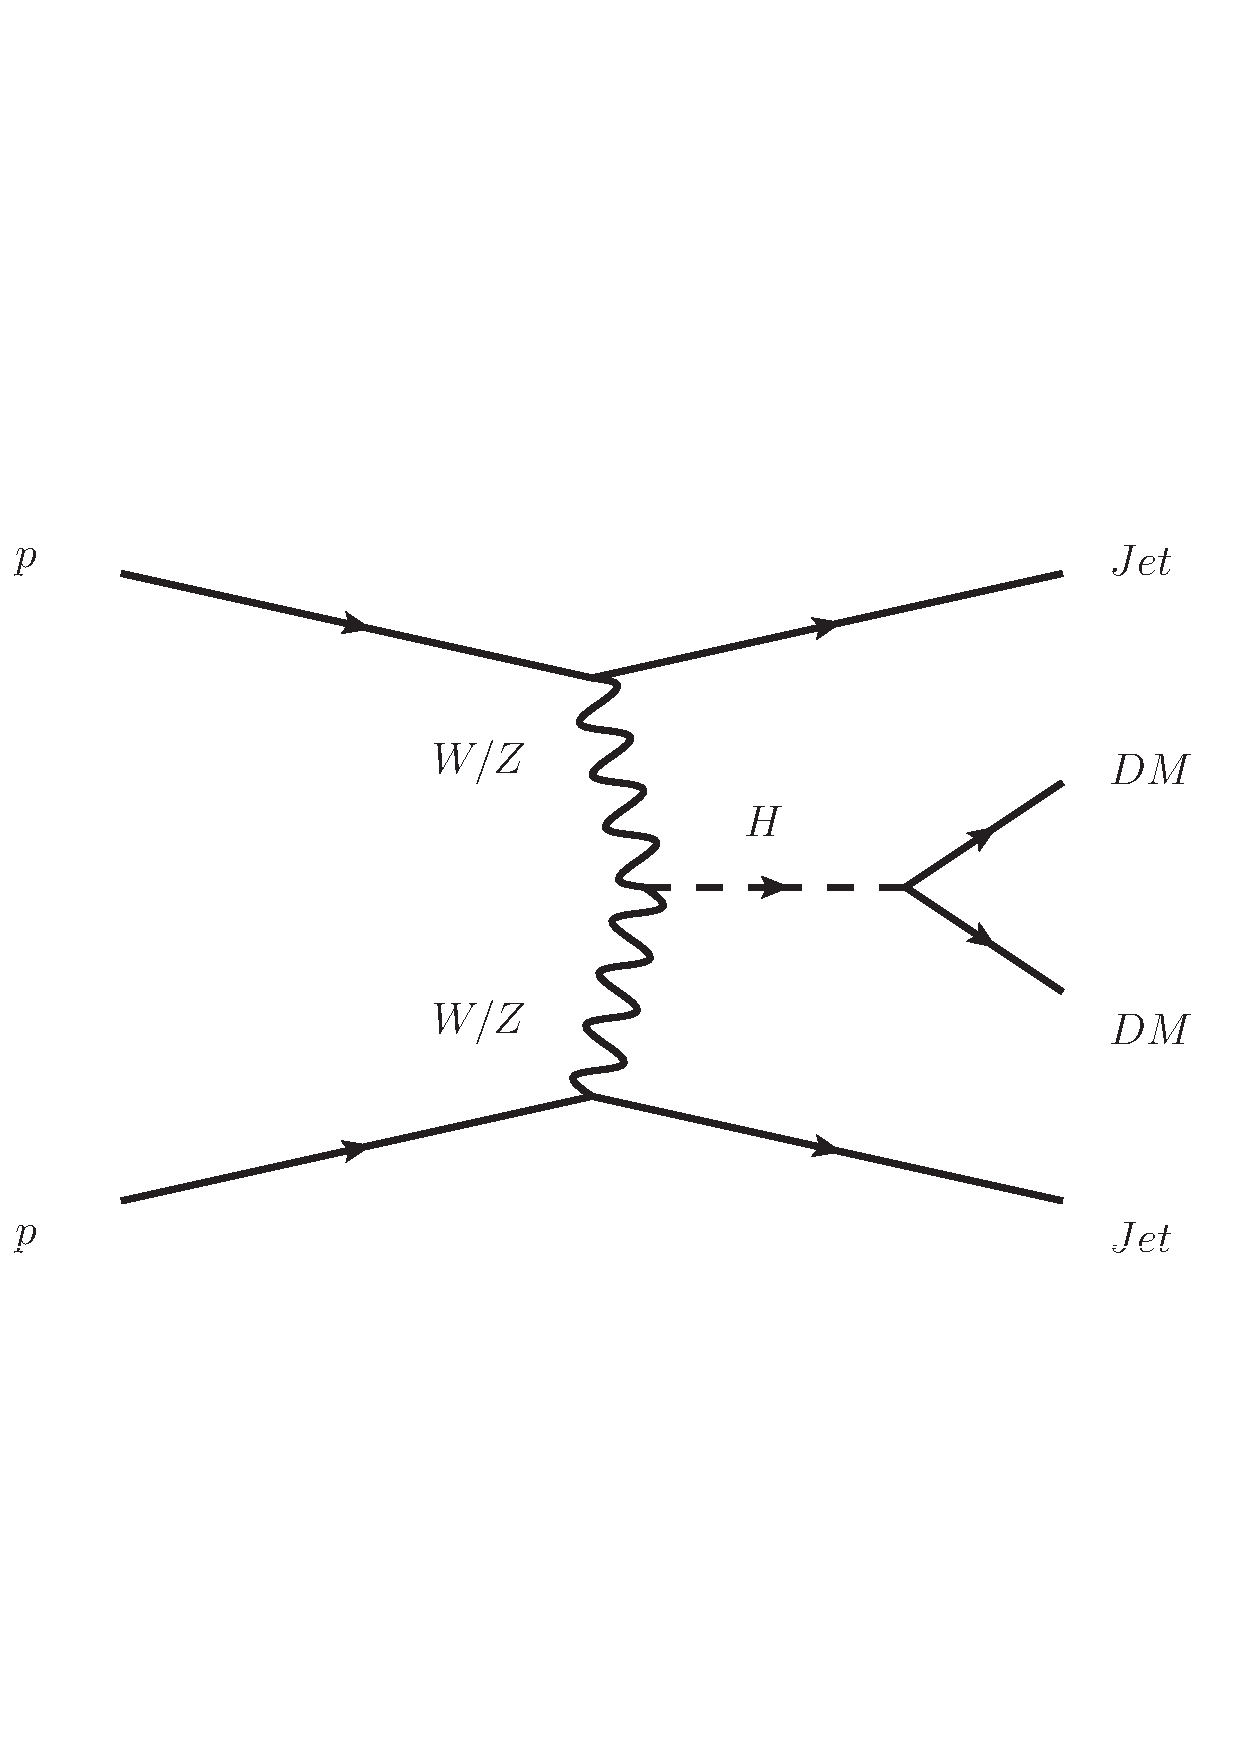
\includegraphics[width=7cm]{pphiggsdmdmjj.pdf}
\end{column}
\begin{column}{.4\textwidth}
\begin{itemize}
\item Interactions are the same as the BSM EFT.
\item Production of Higgs followed by a decay into dark matter.
\end{itemize}
\end{column}
\end{columns}
\end{frame}



\begin{frame}
\frametitle{Phasespace Selection Cuts}
\textcolor{Plum}{\textbf{VBFZ Baseline:}} Jet1PT \textgreater 55 GeV; Jet2PT \textgreater 45 GeV; NumJets $\ge$ 2.
\newline
\newline \textcolor{Plum}{\textbf{VBFZ HighMass:}} Mjj \textgreater 1000 GeV; Jet1PT \textgreater 55 GeV; Jet2PT \textgreater 45 GeV; NumJets $\ge$ 2.
\newline
\newline \textcolor{Plum}{\textbf{VBFZ Search:}} Mjj \textgreater 250 GeV; Jet1PT \textgreater 55 GeV; Jet2PT \textgreater 45 GeV; NumJets $\ge$ 2. 
\newline
\newline \textcolor{Plum}{\textbf{VBFDM:}} Mjj \textgreater 250 GeV; Jet1PT \textgreater 55 GeV; Jet2PT \textgreater 45 GeV; NumJets $\ge$ 2; eta \textless 4.4; MET \textgreater 150 GeV.
\newline
\newline \textcolor{Plum}{\textbf{Monojet:}} Jet1PT \textgreater 100 GeV; NumJets $\ge$ 1; eta \textless 4.4; MET \textgreater 150 GeV.
\newline
\newline \textcolor{Plum}{\textbf{Monojet HighPt:}} Jet1PT \textgreater 250 GeV; NumJets $\ge$ 1; eta \textless 4.4; MET \textgreater 250 GeV.
\newline
\newline \textcolor{Plum}{\textbf{VBFDM OR Monojet:}} VBFDM; Monojet.
\newline
\newline \textcolor{Plum}{\textbf{VBFDM OR Monojet HighPt:}} VBFDM; Monojet HighPt.
\end{frame}

\begin{frame}
\frametitle{Distributions of interest:}
\begin{exampleblock}{Main distributions that have been produced:}
\begin{itemize}
\item Transverse Momentum of Jets, P$_{\text{T}}$(j1) and P$_{\text{T}}$(j2).
\item Dijet Mass, M$_{\text{jj}}$.
\item Missing Transverse Energy,  $\not{E}_{T}$.
\item Difference in Jet Angle $\Delta \phi$.
\item Difference in Jet Pseudorapidity, $\Delta \eta$.
\end{itemize}
\end{exampleblock}
\end{frame}

%------------------------------------------------
\section{Constant Mass} % Sections can be created in order to organize your presentation into discrete blocks, all sections and subsections are automatically printed in the table of contents as an overview of the talk

%------------------------------------------------

\begin{frame}
\frametitle{\small{Distributions for VBFDM OR Monojet Selection, 10 GeV}}
\begin{columns}
\begin{column}{.3\textwidth}
\center{DeltaEta}
\includegraphics[width=4cm, height=3cm]{/Mass10/Absolute/Mass10_DeltaEta_PS_VBFDM_OR_Monojet.pdf}
\center{Mjj}
\includegraphics[width=4cm, height=3cm]{/Mass10/Absolute/Mass10_Mjj_PS_VBFDM_OR_Monojet.pdf}
\end{column}
\begin{column}{.3\textwidth}
\center{DeltaPhi}
\includegraphics[width=4cm, height=3cm]{/Mass10/Absolute/Mass10_DeltaPhi_PS_VBFDM_OR_Monojet.pdf}
\center{Jet1PT}
\includegraphics[width=4cm, height=3cm]{/Mass10/Absolute/Mass10_Jet1PT_PS_VBFDM_OR_Monojet.pdf}
\end{column}
\begin{column}{.3\textwidth}
\center{ETMiss}
\includegraphics[width=4cm, height=3cm]{/Mass10/Absolute/Mass10_ETMiss_PS_VBFDM_OR_Monojet.pdf}
\center{Jet1Eta}
\includegraphics[width=4cm, height=3cm]{/Mass10/Absolute/Mass10_Jet1Eta_PS_VBFDM_OR_Monojet.pdf}
\end{column}
\end{columns}
\end{frame}

\begin{frame}
\frametitle{\small{Distributions for VBFDM OR Monojet HighPt Selection, 10 GeV}}
\begin{columns}
\begin{column}{.3\textwidth}
\center{DeltaEta}
\includegraphics[width=4cm, height=3cm]{/Mass10/Absolute/Mass10_DeltaEta_PS_VBFDM_OR_Monojet_HighPt.pdf}
\center{Mjj}
\includegraphics[width=4cm, height=3cm]{/Mass10/Absolute/Mass10_Mjj_PS_VBFDM_OR_Monojet_HighPt.pdf}
\end{column}
\begin{column}{.3\textwidth}
\center{DeltaPhi}
\includegraphics[width=4cm, height=3cm]{/Mass10/Absolute/Mass10_DeltaPhi_PS_VBFDM_OR_Monojet_HighPt.pdf}
\center{Jet1PT}
\includegraphics[width=4cm, height=3cm]{/Mass10/Absolute/Mass10_Jet1PT_PS_VBFDM_OR_Monojet_HighPt.pdf}
\end{column}
\begin{column}{.3\textwidth}
\center{ETMiss}
\includegraphics[width=4cm, height=3cm]{/Mass10/Absolute/Mass10_ETMiss_PS_VBFDM_OR_Monojet_HighPt.pdf}
\center{Jet1Eta}
\includegraphics[width=4cm, height=3cm]{/Mass10/Absolute/Mass10_Jet1Eta_PS_VBFDM_OR_Monojet_HighPt.pdf}
\end{column}
\end{columns}
\end{frame}

\begin{frame}
\frametitle{\small{Distributions for VBFDM OR Monojet Selection, 100 GeV}}
\begin{columns}
\begin{column}{.3\textwidth}
\center{DeltaEta}
\includegraphics[width=4cm, height=3cm]{/Mass100/Absolute/Mass100_DeltaEta_PS_VBFDM_OR_Monojet.pdf}
\center{Mjj}
\includegraphics[width=4cm, height=3cm]{//Mass100/Absolute/Mass100_Mjj_PS_VBFDM_OR_Monojet.pdf}
\end{column}
\begin{column}{.3\textwidth}
\center{DeltaPhi}
\includegraphics[width=4cm, height=3cm]{/Mass100/Absolute/Mass100_DeltaPhi_PS_VBFDM_OR_Monojet.pdf}
\center{Jet1PT}
\includegraphics[width=4cm, height=3cm]{/Mass100/Absolute/Mass100_Jet1PT_PS_VBFDM_OR_Monojet.pdf}
\end{column}
\begin{column}{.3\textwidth}
\center{ETMiss}
\includegraphics[width=4cm, height=3cm]{/Mass100/Absolute/Mass100_ETMiss_PS_VBFDM_OR_Monojet.pdf}
\center{Jet1Eta}
\includegraphics[width=4cm, height=3cm]{/Mass100/Absolute/Mass100_Jet1Eta_PS_VBFDM_OR_Monojet.pdf}
\end{column}
\end{columns}
\end{frame}

\begin{frame}
\frametitle{\small{Distributions for VBFDM OR Monojet HighPt Selection, 100 GeV}}
\begin{columns}
\begin{column}{.3\textwidth}
\center{DeltaEta}
\includegraphics[width=4cm, height=3cm]{/Mass100/Absolute/Mass100_DeltaEta_PS_VBFDM_OR_Monojet_HighPt.pdf}
\center{Mjj}
\includegraphics[width=4cm, height=3cm]{//Mass100/Absolute/Mass100_Mjj_PS_VBFDM_OR_Monojet_HighPt.pdf}
\end{column}
\begin{column}{.3\textwidth}
\center{DeltaPhi}
\includegraphics[width=4cm, height=3cm]{/Mass100/Absolute/Mass100_DeltaPhi_PS_VBFDM_OR_Monojet_HighPt.pdf}
\center{Jet1PT}
\includegraphics[width=4cm, height=3cm]{/Mass100/Absolute/Mass100_Jet1PT_PS_VBFDM_OR_Monojet_HighPt.pdf}
\end{column}
\begin{column}{.3\textwidth}
\center{ETMiss}
\includegraphics[width=4cm, height=3cm]{/Mass100/Absolute/Mass100_ETMiss_PS_VBFDM_OR_Monojet_HighPt.pdf}
\center{Jet1Eta}
\includegraphics[width=4cm, height=3cm]{/Mass100/Absolute/Mass100_Jet1Eta_PS_VBFDM_OR_Monojet_HighPt.pdf}
\end{column}
\end{columns}
\end{frame}

\begin{frame}
\frametitle{\small{Distributions for VBFDM OR Monojet Selection, 1000 GeV}}
\begin{columns}
\begin{column}{.3\textwidth}
\center{DeltaEta}
\includegraphics[width=4cm, height=3cm]{/Mass1000/Absolute/Mass1000_DeltaEta_PS_VBFDM_OR_Monojet.pdf}
\center{Mjj}
\includegraphics[width=4cm, height=3cm]{//Mass1000/Absolute/Mass1000_Mjj_PS_VBFDM_OR_Monojet.pdf}
\end{column}
\begin{column}{.3\textwidth}
\center{DeltaPhi}
\includegraphics[width=4cm, height=3cm]{/Mass1000/Absolute/Mass1000_DeltaPhi_PS_VBFDM_OR_Monojet.pdf}
\center{Jet1PT}
\includegraphics[width=4cm, height=3cm]{/Mass1000/Absolute/Mass1000_Jet1PT_PS_VBFDM_OR_Monojet.pdf}
\end{column}
\begin{column}{.3\textwidth}
\center{ETMiss}
\includegraphics[width=4cm, height=3cm]{/Mass1000/Absolute/Mass1000_ETMiss_PS_VBFDM_OR_Monojet.pdf}
\center{Jet1Eta}
\includegraphics[width=4cm, height=3cm]{/Mass1000/Absolute/Mass1000_Jet1Eta_PS_VBFDM_OR_Monojet.pdf}
\end{column}
\end{columns}
\end{frame}

\begin{frame}
\frametitle{\small{Distributions for VBFDM OR Monojet HighPt Selection, 1000 GeV}}
\begin{columns}
\begin{column}{.3\textwidth}
\center{DeltaEta}
\includegraphics[width=4cm, height=3cm]{/Mass1000/Absolute/Mass1000_DeltaEta_PS_VBFDM_OR_Monojet_HighPt.pdf}
\center{Mjj}
\includegraphics[width=4cm, height=3cm]{/Mass1000/Absolute/Mass1000_Mjj_PS_VBFDM_OR_Monojet_HighPt.pdf}
\end{column}
\begin{column}{.3\textwidth}
\center{DeltaPhi}
\includegraphics[width=4cm, height=3cm]{/Mass1000/Absolute/Mass1000_DeltaPhi_PS_VBFDM_OR_Monojet_HighPt.pdf}
\center{Jet1PT}
\includegraphics[width=4cm, height=3cm]{/Mass1000/Absolute/Mass1000_Jet1PT_PS_VBFDM_OR_Monojet_HighPt.pdf}
\end{column}
\begin{column}{.3\textwidth}
\center{ETMiss}
\includegraphics[width=4cm, height=3cm]{/Mass1000/Absolute/Mass1000_ETMiss_PS_VBFDM_OR_Monojet_HighPt.pdf}
\center{Jet1Eta}
\includegraphics[width=4cm, height=3cm]{/Mass1000/Absolute/Mass1000_Jet1Eta_PS_VBFDM_OR_Monojet_HighPt.pdf}
\end{column}
\end{columns}
\end{frame}

\begin{frame}
\frametitle{Scaled Cross-section:}
\begin{exampleblock}{Phase Space Key:}
1 = VBFZ Baseline; 2 = VBFZ HighMass; 3 = VBFZ Baseline; 4 = VBFDM; \newline 5 = Monojet; 6 = Monojet HighPt; 7 = VBFDM OR Monojet; \newline8 = VBFDM OR Monojet HighPt
\end{exampleblock}
\vspace{0.75cm}
\begin{columns}
\begin{column}{.3\textwidth}
\center{DM Mass 10 GeV}
\includegraphics[width=4cm, height=3cm]{/Mass10/Absolute/Mass10_Count_for_All_PS_CrossSection.pdf}
\end{column}
\begin{column}{.3\textwidth}
\center{DM Mass 100 GeV}
\includegraphics[width=4cm, height=3cm]{/Mass100/Absolute/Mass100_Count_for_All_PS_CrossSection.pdf}
\end{column}
\begin{column}{.3\textwidth}
\center{DM Mass 1000 GeV}
\includegraphics[width=4cm, height=3cm]{/Mass1000/Absolute/Mass1000_Count_for_All_PS_CrossSection.pdf}
\end{column}
\end{columns}
\end{frame}

%------------------------------------------------
\section{Constant Dimension} % Sections can be created in order to organize your presentation into discrete blocks, all sections and subsections are automatically printed in the table of contents as an overview of the talk

%------------------------------------------------

\begin{frame}
\frametitle{Distributions for D5a, VBFDM Selection}
\begin{columns}
\begin{column}{.3\textwidth}
\center{DeltaEta}
\includegraphics[width=4cm, height=3cm]{/D5a/Absolute/D5a_DeltaEta_PS_VBFDM.pdf}
\center{Mjj}
\includegraphics[width=4cm, height=3cm]{D5a/Absolute/D5a_Mjj_PS_VBFDM.pdf}
\end{column}
\begin{column}{.3\textwidth}
\center{DeltaPhi}
\includegraphics[width=4cm, height=3cm]{D5a/Absolute/D5a_DeltaPhi_PS_VBFDM.pdf}
\center{Jet1PT}
\includegraphics[width=4cm, height=3cm]{D5a/Absolute/D5a_Jet1PT_PS_VBFDM.pdf}
\end{column}
\begin{column}{.3\textwidth}
\center{ETMiss}
\includegraphics[width=4cm, height=3cm]{D5a/Absolute/D5a_ETMiss_PS_VBFDM.pdf}
\center{Jet1Eta}
\includegraphics[width=4cm, height=3cm]{D5a/Absolute/D5a_Jet1Eta_PS_VBFDM.pdf}
\end{column}
\end{columns}
\end{frame}

\begin{frame}
\frametitle{Distributions for D5b, VBFDM Selection}
\begin{columns}
\begin{column}{.3\textwidth}
\center{DeltaEta}
\includegraphics[width=4cm, height=3cm]{/D5b/Absolute/D5b_DeltaEta_PS_VBFDM.pdf}
\center{Mjj}
\includegraphics[width=4cm, height=3cm]{D5b/Absolute/D5b_Mjj_PS_VBFDM.pdf}
\end{column}
\begin{column}{.3\textwidth}
\center{DeltaPhi}
\includegraphics[width=4cm, height=3cm]{/D5b/Absolute/D5b_DeltaPhi_PS_VBFDM.pdf}
\center{Jet1PT}
\includegraphics[width=4cm, height=3cm]{/D5b/Absolute/D5b_Jet1PT_PS_VBFDM.pdf}
\end{column}
\begin{column}{.3\textwidth}
\center{ETMiss}
\includegraphics[width=4cm, height=3cm]{D5b/Absolute/D5b_ETMiss_PS_VBFDM.pdf}
\center{Jet1Eta}
\includegraphics[width=4cm, height=3cm]{D5b/Absolute/D5b_Jet1Eta_PS_VBFDM.pdf}
\end{column}
\end{columns}
\end{frame}

\begin{frame}
\frametitle{Distributions for D5c, VBFDM Selection}
\begin{columns}
\begin{column}{.3\textwidth}
\center{DeltaEta}
\includegraphics[width=4cm, height=3cm]{/D5c/Absolute/D5c_DeltaEta_PS_VBFDM.pdf}
\center{Mjj}
\includegraphics[width=4cm, height=3cm]{/D5c/Absolute/D5c_Mjj_PS_VBFDM.pdf}
\end{column}
\begin{column}{.3\textwidth}
\center{DeltaPhi}
\includegraphics[width=4cm, height=3cm]{/D5c/Absolute/D5c_DeltaPhi_PS_VBFDM.pdf}
\center{Jet1PT}
\includegraphics[width=4cm, height=3cm]{/D5c/Absolute/D5c_Jet1PT_PS_VBFDM.pdf}
\end{column}
\begin{column}{.3\textwidth}
\center{ETMiss}
\includegraphics[width=4cm, height=3cm]{/D5c/Absolute/D5c_ETMiss_PS_VBFDM.pdf}
\center{Jet1Eta}
\includegraphics[width=4cm, height=3cm]{D5c/Absolute/D5c_Jet1Eta_PS_VBFDM.pdf}
\end{column}
\end{columns}
\end{frame}

\begin{frame}
\frametitle{Distributions for D5d, VBFDM Selection}
\begin{columns}
\begin{column}{.3\textwidth}
\center{DeltaEta}
\includegraphics[width=4cm, height=3cm]{/D5d/Absolute/D5d_DeltaEta_PS_VBFDM.pdf}
\center{Mjj}
\includegraphics[width=4cm, height=3cm]{/D5d/Absolute/D5d_Mjj_PS_VBFDM.pdf}
\end{column}
\begin{column}{.3\textwidth}
\center{DeltaPhi}
\includegraphics[width=4cm, height=3cm]{/D5d/Absolute/D5d_DeltaPhi_PS_VBFDM.pdf}
\center{Jet1PT}
\includegraphics[width=4cm, height=3cm]{/D5d/Absolute/D5d_Jet1PT_PS_VBFDM.pdf}
\end{column}
\begin{column}{.3\textwidth}
\center{ETMiss}
\includegraphics[width=4cm, height=3cm]{/D5d/Absolute/D5d_ETMiss_PS_VBFDM.pdf}
\center{Jet1Eta}
\includegraphics[width=4cm, height=3cm]{D5d/Absolute/D5d_Jet1Eta_PS_VBFDM.pdf}
\end{column}
\end{columns}
\end{frame}

\begin{frame}
\frametitle{Distributions for D6a, VBFDM Selection}
\begin{columns}
\begin{column}{.3\textwidth}
\center{DeltaEta}
\includegraphics[width=4cm, height=3cm]{/D6a/Absolute/D6a_DeltaEta_PS_VBFDM.pdf}
\center{Mjj}
\includegraphics[width=4cm, height=3cm]{/D6a/Absolute/D6a_Mjj_PS_VBFDM.pdf}
\end{column}
\begin{column}{.3\textwidth}
\center{DeltaPhi}
\includegraphics[width=4cm, height=3cm]{/D6a/Absolute/D6a_DeltaPhi_PS_VBFDM.pdf}
\center{Jet1PT}
\includegraphics[width=4cm, height=3cm]{/D6a/Absolute/D6a_Jet1PT_PS_VBFDM.pdf}
\end{column}
\begin{column}{.3\textwidth}
\center{ETMiss}
\includegraphics[width=4cm, height=3cm]{/D6a/Absolute/D6a_ETMiss_PS_VBFDM.pdf}
\center{Jet1Eta}
\includegraphics[width=4cm, height=3cm]{D6a/Absolute/D6a_Jet1Eta_PS_VBFDM.pdf}
\end{column}
\end{columns}
\end{frame}

\begin{frame}
\frametitle{Distributions for D6b, VBFDM Selection}
\begin{columns}
\begin{column}{.3\textwidth}
\center{DeltaEta}
\includegraphics[width=4cm, height=3cm]{/D6b/Absolute/D6b_DeltaEta_PS_VBFDM.pdf}
\center{Mjj}
\includegraphics[width=4cm, height=3cm]{/D6b/Absolute/D6b_Mjj_PS_VBFDM.pdf}
\end{column}
\begin{column}{.3\textwidth}
\center{DeltaPhi}
\includegraphics[width=4cm, height=3cm]{/D6b/Absolute/D6b_DeltaPhi_PS_VBFDM.pdf}
\center{Jet1PT}
\includegraphics[width=4cm, height=3cm]{/D6b/Absolute/D6b_Jet1PT_PS_VBFDM.pdf}
\end{column}
\begin{column}{.3\textwidth}
\center{ETMiss}
\includegraphics[width=4cm, height=3cm]{/D6b/Absolute/D6b_ETMiss_PS_VBFDM.pdf}
\center{Jet1Eta}
\includegraphics[width=4cm, height=3cm]{D6b/Absolute/D6b_Jet1Eta_PS_VBFDM.pdf}
\end{column}
\end{columns}
\end{frame}

\begin{frame}
\frametitle{Distributions for D7a, VBFDM Selection}
\begin{columns}
\begin{column}{.3\textwidth}
\center{DeltaEta}
\includegraphics[width=4cm, height=3cm]{/D7a/Absolute/D7a_DeltaEta_PS_VBFDM.pdf}
\center{Mjj}
\includegraphics[width=4cm, height=3cm]{/D7a/Absolute/D7a_Mjj_PS_VBFDM.pdf}
\end{column}
\begin{column}{.3\textwidth}
\center{DeltaPhi}
\includegraphics[width=4cm, height=3cm]{/D7a/Absolute/D7a_DeltaPhi_PS_VBFDM.pdf}
\center{Jet1PT}
\includegraphics[width=4cm, height=3cm]{/D7a/Absolute/D7a_Jet1PT_PS_VBFDM.pdf}
\end{column}
\begin{column}{.3\textwidth}
\center{ETMiss}
\includegraphics[width=4cm, height=3cm]{/D7a/Absolute/D7a_ETMiss_PS_VBFDM.pdf}
\center{Jet1Eta}
\includegraphics[width=4cm, height=3cm]{D7a/Absolute/D7a_Jet1Eta_PS_VBFDM.pdf}
\end{column}
\end{columns}
\end{frame}

\begin{frame}
\frametitle{Distributions for D7b, VBFDM Selection}
\begin{columns}
\begin{column}{.3\textwidth}
\center{DeltaEta}
\includegraphics[width=4cm, height=3cm]{/D7b/Absolute/D7b_DeltaEta_PS_VBFDM.pdf}
\center{Mjj}
\includegraphics[width=4cm, height=3cm]{/D7b/Absolute/D7b_Mjj_PS_VBFDM.pdf}
\end{column}
\begin{column}{.3\textwidth}
\center{DeltaPhi}
\includegraphics[width=4cm, height=3cm]{/D7b/Absolute/D7b_DeltaPhi_PS_VBFDM.pdf}
\center{Jet1PT}
\includegraphics[width=4cm, height=3cm]{/D7b/Absolute/D7b_Jet1PT_PS_VBFDM.pdf}
\end{column}
\begin{column}{.3\textwidth}
\center{ETMiss}
\includegraphics[width=4cm, height=3cm]{/D7b/Absolute/D7b_ETMiss_PS_VBFDM.pdf}
\center{Jet1Eta}
\includegraphics[width=4cm, height=3cm]{D7b/Absolute/D7b_Jet1Eta_PS_VBFDM.pdf}
\end{column}
\end{columns}
\end{frame}

\begin{frame}
\frametitle{Distributions for D7c, VBFDM Selection}
\begin{columns}
\begin{column}{.3\textwidth}
\center{DeltaEta}
\includegraphics[width=4cm, height=3cm]{/D7c/Absolute/D7c_DeltaEta_PS_VBFDM.pdf}
\center{Mjj}
\includegraphics[width=4cm, height=3cm]{/D7c/Absolute/D7c_Mjj_PS_VBFDM.pdf}
\end{column}
\begin{column}{.3\textwidth}
\center{DeltaPhi}
\includegraphics[width=4cm, height=3cm]{/D7c/Absolute/D7c_DeltaPhi_PS_VBFDM.pdf}
\center{Jet1PT}
\includegraphics[width=4cm, height=3cm]{/D7c/Absolute/D7c_Jet1PT_PS_VBFDM.pdf}
\end{column}
\begin{column}{.3\textwidth}
\center{ETMiss}
\includegraphics[width=4cm, height=3cm]{/D7c/Absolute/D7c_ETMiss_PS_VBFDM.pdf}
\center{Jet1Eta}
\includegraphics[width=4cm, height=3cm]{D7c/Absolute/D7c_Jet1Eta_PS_VBFDM.pdf}
\end{column}
\end{columns}
\end{frame}

\begin{frame}
\frametitle{Distributions for D7d, VBFDM Selection}
\begin{columns}
\begin{column}{.3\textwidth}
\center{DeltaEta}
\includegraphics[width=4cm, height=3cm]{/D7d/Absolute/D7d_DeltaEta_PS_VBFDM.pdf}
\center{Mjj}
\includegraphics[width=4cm, height=3cm]{/D7d/Absolute/D7d_Mjj_PS_VBFDM.pdf}
\end{column}
\begin{column}{.3\textwidth}
\center{DeltaPhi}
\includegraphics[width=4cm, height=3cm]{/D7d/Absolute/D7d_DeltaPhi_PS_VBFDM.pdf}
\center{Jet1PT}
\includegraphics[width=4cm, height=3cm]{/D7d/Absolute/D7d_Jet1PT_PS_VBFDM.pdf}
\end{column}
\begin{column}{.3\textwidth}
\center{ETMiss}
\includegraphics[width=4cm, height=3cm]{/D7d/Absolute/D7d_ETMiss_PS_VBFDM.pdf}
\center{Jet1Eta}
\includegraphics[width=4cm, height=3cm]{D7d/Absolute/D7d_Jet1Eta_PS_VBFDM.pdf}
\end{column}
\end{columns}
\end{frame}

%------------------------------------------------
\section{Next Steps} % Sections can be created in order to organize your presentation into discrete blocks, all sections and subsections are automatically printed in the table of contents as an overview of the talk

%------------------------------------------------

\begin{frame}
\frametitle{Next Steps:}
\begin{itemize}
\item Make 2D plots from the distributions
\item Look at invisible Higgs validation of Sherpa.
\item Add three jet contributions.
\item Make 2D plots of rates in mass and $\Lambda$.
\item Any other thoughts?
\end{itemize}
\end{frame}







\end{document} 